% ============================================================================
% §6 RESULTADOS
% ============================================================================
\section{Resultados}
\label{sec:resultados}

Esta sección presenta los resultados del \emph{backtest} sobre TSLA, organiza las cinco figuras generadas por el programa e interpreta cada una en el contexto de las secciones anteriores.

% ----------------------------------------------------------------------------
\subsection{Configuración experimental}
\label{subsec:config-experimental}

Los resultados que se muestran a continuación corresponden a la siguiente configuración:

\begin{center}
\begin{tabular}{ll}
\toprule
Activo & TSLA (Tesla, Inc.) \\
Periodo & 2 años ($\approx 506$ sesiones) \\
Capital inicial & 10\,000\,\$ \\
\texttt{ITERACIONES} & 5\,000 \\
\texttt{DIAS\_ROLLOUT} & 60 \\
\texttt{VENTANA\_CALIB} & 60 días \\
\texttt{SEMILLA} & 42 \\
\bottomrule
\end{tabular}
\end{center}

\begin{observacion}[Discrepancia en \texttt{ITERACIONES}]
\label{obs:iteraciones}
Las figuras presentadas en esta sección fueron generadas con \texttt{ITERACIONES}~$= 5\,000$, un valor superior al \texttt{ITERACIONES}~$= 1\,000$ declarado en el código actual del archivo \texttt{mcts\_simple\_TSLA.py}. En virtud del Teorema~\ref{teorema:error-mc}, el aumento de iteraciones reduce el error del estimador a razón de $\mathcal{O}(n^{-1/2})$: pasar de 1\,000 a 5\,000 iteraciones divide el error típico por $\sqrt{5} \approx 2{.}24$, produciendo decisiones más fiables aunque a mayor coste computacional.
\end{observacion}

\paragraph{Contexto del mercado.} El periodo analizado cubre aproximadamente dos años de cotización de TSLA y abarca un régimen de mercado extremadamente volátil. El precio inicia en torno a los $150$\,\$, asciende hasta un máximo de $\approx 480$\,\$ (sesión $\approx 170$), sufre una corrección severa hasta los $\approx 120$\,\$ (sesión $\approx 230$), recupera el máximo anterior ($\approx 480$\,\$, sesión $\approx 420$) y cierra el periodo alrededor de los $350$\,\$. La volatilidad diaria media de los log-retornos es del $1{.}903\,\%$ (equivalente a una volatilidad anualizada de $\approx 30{.}2\,\%$), clasificable como muy alta para un activo individual. Este entorno prueba de forma exigente la capacidad adaptativa del agente.

% ----------------------------------------------------------------------------
\subsection{Resultados globales}
\label{subsec:resultados-globales}

La Tabla~\ref{tab:resultados-globales} recoge las métricas de evaluación (definidas en §\ref{subsec:metricas}) para la estrategia MCTS y la referencia Buy \& Hold.

\begin{table}[H]
\centering
\caption{Métricas comparativas MCTS vs.\ Buy \& Hold (TSLA, 2 años).}
\label{tab:resultados-globales}
\begin{tabular}{lcc}
\toprule
\textbf{Métrica} & \textbf{MCTS} & \textbf{Buy \& Hold} \\
\midrule
ROI total             & $\approx +240\,\%$ & $\approx +100\,\%$ \\
Retorno diario medio  & $+0{.}302\,\%$     & $+0{.}232\,\%$ \\
Desv.\ típica diaria  & $3{.}065\,\%$      & $1{.}903\,\%$ \\
Sharpe anualizado     & $\approx 1{.}56$   & $\approx 1{.}93$ \\
Días con retorno $>0$ & 216 (43{.}3\,\%)  & 254 (50{.}9\,\%) \\
Drawdown máximo       & $\approx -10\,\%$  & —\\
Alfa final (vs.\ B\&H)& $\approx +40\,\%$ & — \\
Drawdown máximo del alfa & $\approx -35\,\%$ & — \\
\bottomrule
\end{tabular}
\end{table}

Los resultados revelan una tensión interesante: MCTS obtiene un ROI total significativamente superior al de B\&H ($+240\,\%$ frente a $+100\,\%$), pero a costa de una mayor volatilidad diaria ($3{.}065\,\%$ frente a $1{.}903\,\%$), lo que resulta en un ratio de Sharpe \emph{inferior} ($1{.}56$ frente a $1{.}93$). En términos ajustados por riesgo, B\&H es la estrategia más eficiente; en términos de retorno absoluto, MCTS domina claramente.

% ----------------------------------------------------------------------------
\subsection{Evolución de la cartera, alfa y drawdown}
\label{subsec:evolucion-cartera}

\begin{figure}[H]
    \centering
    
\includegraphics[width=\linewidth]{figuras/mcts_simple_resultado.png}
    \caption{Panel de resultados. De arriba abajo: (1) precio de TSLA con señales COMPRAR/VENDER; (2) evolución de la cartera (base~100) MCTS vs.\ B\&H; (3) alfa relativa MCTS vs.\ B\&H; (4) drawdown de la cartera MCTS (rojo) y drawdown del alfa (morado).}
    \label{fig:resultado-principal}
\end{figure}

La Figura~\ref{fig:resultado-principal} contiene cuatro paneles que deben leerse conjuntamente.

\paragraph{Panel 1 — Señales de decisión.} El agente MCTS alterna entre compras y ventas a lo largo de todo el periodo. En el tramo bajista (sesiones $\approx 150$--$230$) predominan las señales de venta (triángulos rojos), y en los tramos alcistas predominan las compras (triángulos verdes). Este comportamiento refleja la capacidad del algoritmo de detectar, mediante los rollouts GBM calibrados sobre los últimos 60 días, si el régimen actual es alcista o bajista.

\paragraph{Panel 2 — Evolución de la cartera.} La cartera MCTS (azul) y B\&H (naranja) parten de la misma base 100. La separación más notable ocurre en las sesiones $150$--$250$: mientras B\&H cae en picado con la corrección de TSLA, MCTS mantiene su valor gracias a haberse retirado del mercado (véase §\ref{subsec:exposicion}). Al final del periodo, MCTS alcanza una base $\approx 340$ frente a $\approx 200$ de B\&H, lo que equivale a los ROI de la Tabla~\ref{tab:resultados-globales}.

\paragraph{Panel 3 — Alfa relativa.} El alfa $\alpha_t = V_t^{\text{mcts}}/V_t^{\text{bah}} - 1$ es positiva (verde) durante la mayor parte del periodo, lo que indica que MCTS supera de forma persistente a B\&H. El alfa sube hasta $\approx +80\,\%$ en los días posteriores al mínimo de precio, precisamente cuando el mercado está recuperándose y la cartera B\&H arrastra el efecto de la caída, mientras que MCTS había preservado capital.

\paragraph{Panel 4 — Drawdown de la cartera y del alfa.} El drawdown máximo de la cartera MCTS es de $\approx -10\,\%$, muy moderado dado el nivel de volatilidad de TSLA. El drawdown del alfa llega a $\approx -35\,\%$: hay un periodo (sesiones $\approx 350$--$450$) en que MCTS queda temporalmente rezagado respecto a B\&H, probablemente por haberse retirado del mercado durante una fase alcista continuada.

% ----------------------------------------------------------------------------
\subsection{Exposición dinámica al activo}
\label{subsec:exposicion}

\begin{figure}[H]
    \centering
    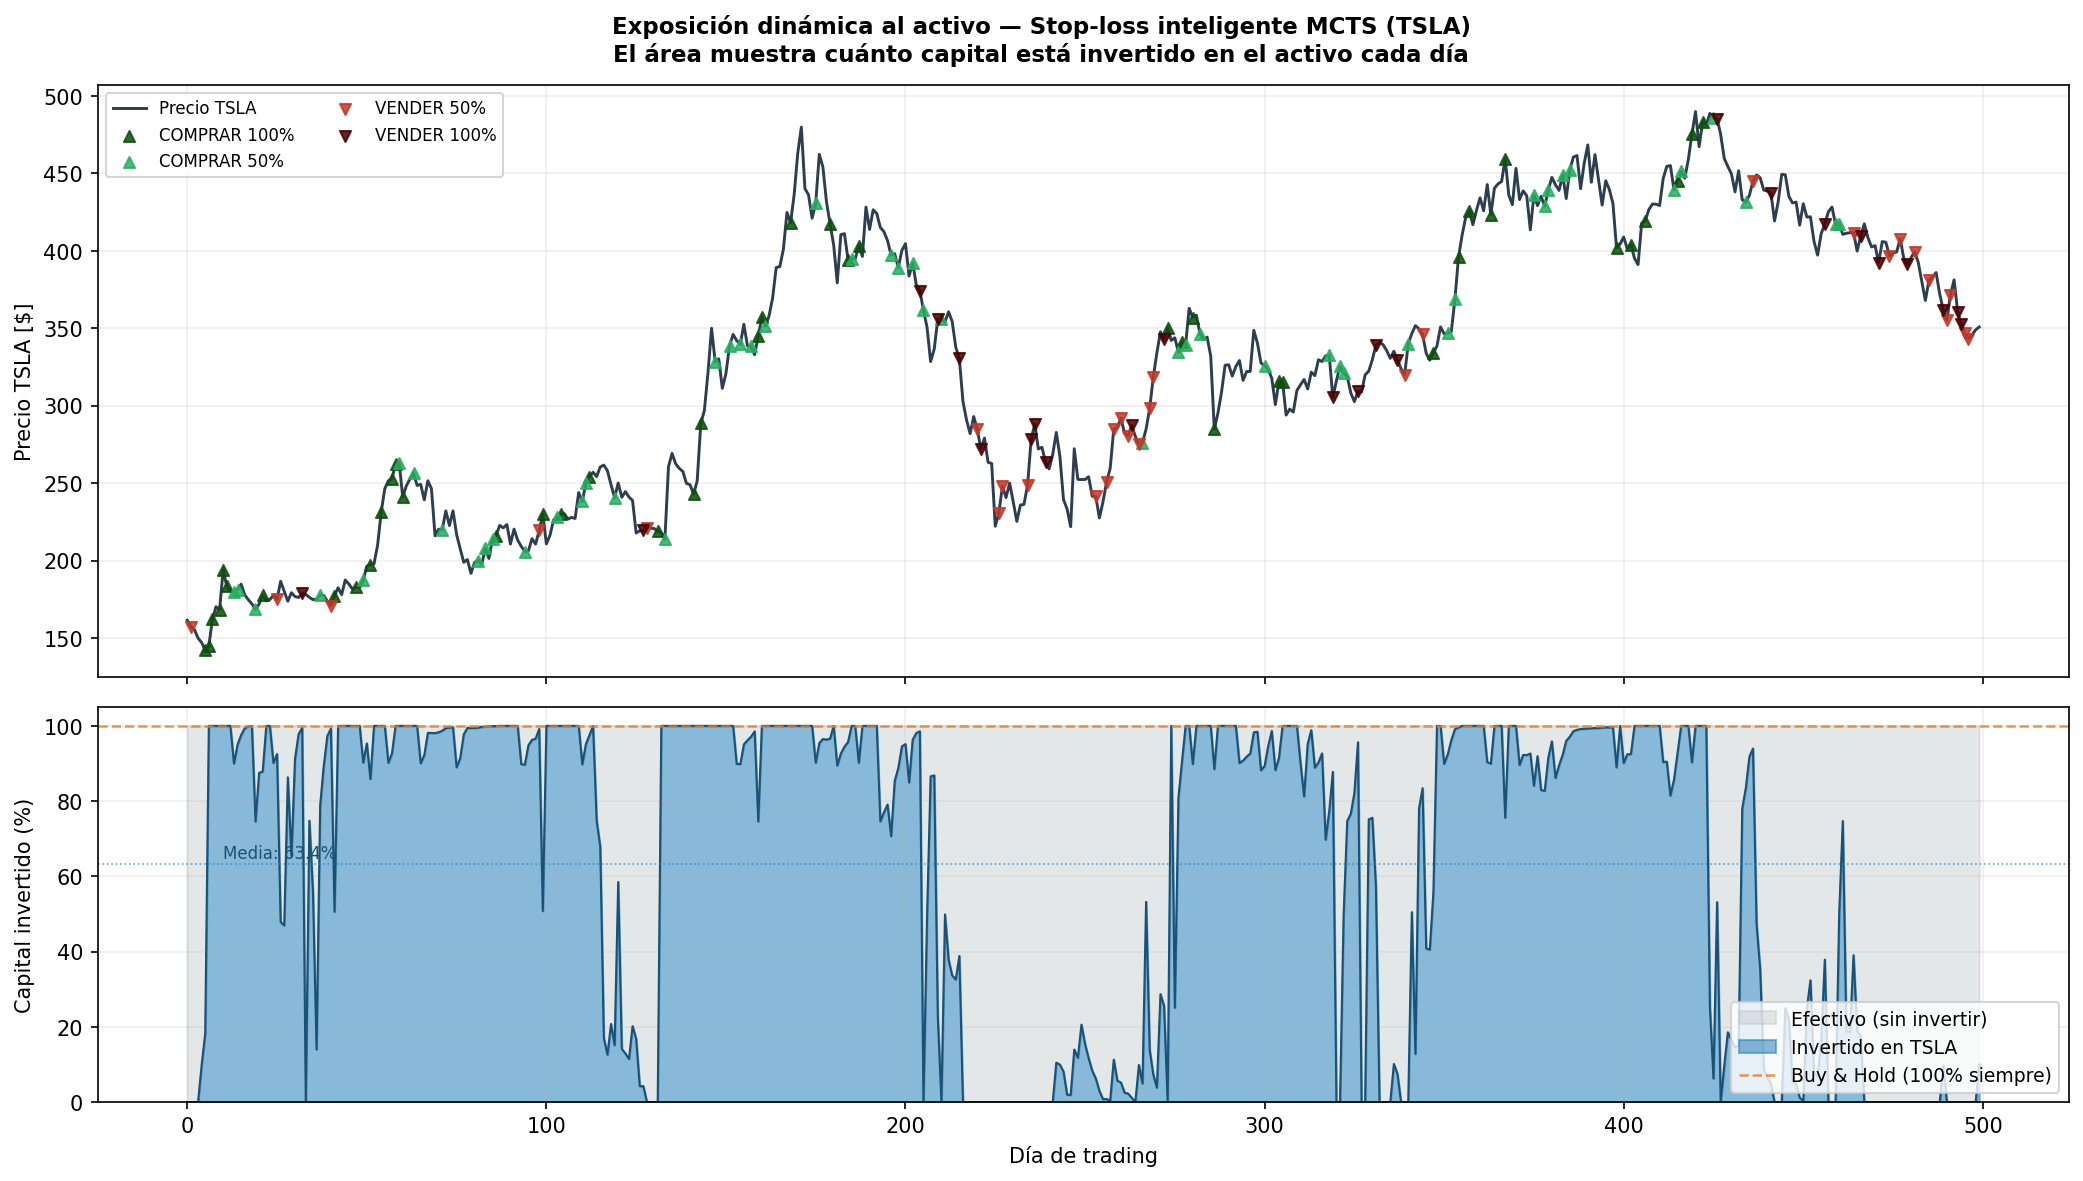
\includegraphics[width=\linewidth]{figuras/mcts_exposicion_dinamica.png}
    \caption{Exposición dinámica. Arriba: precio de TSLA con señales. Abajo: porcentaje del capital invertido en TSLA (azul) y referencia B\&H al 100\,\% (gris).}
    \label{fig:exposicion}
\end{figure}

La Figura~\ref{fig:exposicion} muestra que la política aprendida por MCTS es esencialmente \emph{binaria}: alterna entre exposición plena (100\,\% invertido, $\approx$~\texttt{COMPRAR\_100}) y exposición nula (0\,\% invertido, $\approx$~\texttt{VENDER\_100}), con pocas posiciones fraccionarias intermedias. El periodo en efectivo más prolongado coincide exactamente con la gran corrección de TSLA (sesiones $\approx 150$--$230$), lo que explica el comportamiento favorable del panel 2. Esta política de \emph{timing} de mercado es posible gracias al GBM calibrado con ventana móvil: cuando la volatilidad estimada es alta y la deriva negativa, los rollouts penalizan las posiciones largas.

% ----------------------------------------------------------------------------
\subsection{Ranking de acciones}
\label{subsec:ranking}

\begin{figure}[H]
    \centering
    
\includegraphics[width=0.85\linewidth]{figuras/mcts_convergencia_ucb.png}
    \caption{Convergencia UCB1 en un día representativo (TSLA). Cada línea muestra la recompensa media acumulada $Q(a)/N(a)$ para cada acción a lo largo de las 5\,000 iteraciones.}
    \label{fig:convergencia-ucb}
\end{figure}

La Figura~\ref{fig:convergencia-ucb} permite verificar empíricamente el objetivo~(O5): la validación de la cota $\mathcal{O}(n^{-1/2})$ del Teorema~\ref{teorema:error-mc}. En las primeras $\approx 100$ iteraciones, las líneas oscilan ampliamente (error grande, pocas muestras). A partir de $\approx 500$ iteraciones la convergencia es ya visible, y en torno a $\approx 1\,000$ todas las líneas se han estabilizado. El comportamiento de la envolvente exterior, que decrece en amplitud proporcional a $1/\sqrt{n}$, es coherente con la cota teórica. La separación definitiva entre acciones (las de tipo COMPRAR\_ claramente por encima de VENDER\_ y MANTENER) indica que el árbol, en ese día concreto, ha identificado correctamente el régimen alcista del mercado.

% ----------------------------------------------------------------------------
\subsection{Distribución de retornos}
\label{subsec:distribucion-retornos}

\begin{figure}[H]
    \centering
    
\includegraphics[width=0.85\linewidth]{figuras/mcts_violin_retornos.png}
    \caption{Distribución de retornos diarios. MCTS (azul) vs.\ B\&H (naranja). Las cajas internas indican el rango intercuartílico; los extremos de los violines señalan los valores extremos.}
    \label{fig:violin}
\end{figure}

La Figura~\ref{fig:violin} muestra la distribución empírica completa de los retornos diarios de ambas estrategias. Dos características son inmediatamente visibles:

\begin{itemize}
    \item \textbf{Mayor dispersión de MCTS.} La distribución MCTS tiene colas más anchas: mínimo $-12{.}914\,\%$, máximo $+21{.}919\,\%$, frente a $-22{.}690\,\%$ y $+0{.}724\,\%$ de B\&H respectivamente. La asimetría positiva marcada de MCTS (cola derecha larga) es consecuencia de los días en que el agente está completamente invertido en un mercado fuertemente alcista.
    \item \textbf{Mediana de MCTS en cero.} La mediana de MCTS es $0{.}000\,\%$, frente a $+0{.}036\,\%$ de B\&H. Esto refleja que el agente pasa muchos días en efectivo (retorno exactamente nulo), lo que comprime la mediana sin afectar a la media, que sigue siendo superior ($+0{.}302\,\%$ frente a $+0{.}232\,\%$).
\end{itemize}

La forma de ambos violines es coherente con la distribución log-normal predicha por el modelo GBM de §\ref{subsec:gbm}: la concentración central con colas simétricas en log-retorno corresponde a una distribución de precios log-normal.

% ----------------------------------------------------------------------------
\subsection{Lectura integrada}
\label{subsec:lectura-integrada}

Los seis paneles de resultados cuentan una historia coherente. TSLA presentó durante el periodo un entorno de altísima volatilidad con una corrección severa de $\approx 75\,\%$ seguida de una recuperación de similar magnitud. En este entorno, el algoritmo MCTS, calibrando el GBM sobre ventana móvil, aprendió iteración a iteración (Figura~\ref{fig:convergencia-ucb}) que la acción óptima era retirarse del mercado durante la corrección y reentrar en la recuperación. El resultado es un ROI total de $\approx +240\,\%$ frente a $\approx +100\,\%$ de B\&H, con un drawdown máximo de solo $-10\,\%$, a cambio de una mayor volatilidad diaria y un Sharpe inferior. La Sección~\ref{sec:discusion} discute las implicaciones y las limitaciones de estas conclusiones.
